% speech-affect-lab: technical report.
% Build:  lualatex report && lualatex report   (LuaLaTeX is required by florilegium)
\documentclass[11pt,a4paper]{article}

% ---------------------------------------------------------------- layout & fonts
\usepackage[a4paper,margin=2.4cm,top=2.3cm,bottom=2.6cm]{geometry}
\usepackage{amsmath}
\usepackage{libertinus}
\usepackage{microtype}
\usepackage[english]{babel}
\usepackage{booktabs,tabularx,multirow}
\usepackage{graphicx}
\usepackage[font=small,labelfont=bf,skip=4pt]{caption}
\usepackage{subcaption}
\usepackage[section]{placeins}
\usepackage{xcolor}
\usepackage{enumitem}
\setlist{itemsep=1pt,topsep=3pt}
\usepackage{tikz}
\usetikzlibrary{positioning,arrows.meta,calc,fit,backgrounds}
\usepackage[numbers,sort&compress]{natbib}
\usepackage[colorlinks=true,linkcolor=seriesA,citecolor=seriesA,urlcolor=seriesA]{hyperref}
\usepackage[capitalise,noabbrev]{cleveref}

% Florilegium: mathematical floral margin, drawn on the title page only.
\usepackage[grown,nomargin,theme=math,density=0.45,intensity=0.55]{florilegium}
\definecolor{ink}{HTML}{2A78D6}
\definecolor{accent}{HTML}{EB6834}

\definecolor{seriesA}{HTML}{2A78D6}  % WavLM
\definecolor{seriesB}{HTML}{EB6834}  % HuBERT / eGeMAPS
\definecolor{muted}{HTML}{6B6A63}
\definecolor{gridc}{HTML}{E4E3DC}

\newcommand{\pp}{\,pp}
\newcommand{\ci}[3]{#1\,{\color{muted}\footnotesize[#2;\,#3]}}
\newcommand{\WavLM}{WavLM}
\newcommand{\HuBERT}{HuBERT}

\hypersetup{pdftitle={Frozen self-supervised speech encoders for speaker-independent emotion recognition},
  pdfauthor={Maksym Sokolnytskyi}}

\begin{document}

% ================================================================ title page
\newgeometry{left=5.2cm,right=2.4cm,top=3cm,bottom=2.6cm}
\makeatletter
\AddToShipoutPictureBG*{\AtPageLowerLeft{\put(-\hoffset,\voffset){\florilegium@growngarden}}}
\makeatother
\thispagestyle{empty}
\begin{flushleft}
{\small\color{muted}\textsc{technical report} \hfill November 2026}\par
\vspace{1.6cm}
{\LARGE\bfseries Frozen self-supervised speech encoders\\[3pt] for speaker-independent emotion recognition:\par}
\vspace{6pt}
{\large layers, telephone robustness, CPU deployment,\\ and the geometry of emotion representations\par}
\vspace{1.0cm}
{\large Maksym Sokolnytskyi}\par
{\small\color{muted}\url{https://github.com/MaksymSokolnytskyi/speech-affect-lab}}\par
\vspace{1.2cm}
\end{flushleft}

\noindent\textbf{Abstract.}\enspace
We study how much emotion a \emph{frozen} self-supervised speech encoder exposes to a linear
classifier, and what happens to it under the conditions of a telephone line and a CPU budget.
On CREMA-D (7{,}442 clips, 91 actors, six emotions) with nested speaker-independent
cross-validation, a logistic-regression probe on mean-pooled hidden states reaches an
unweighted average recall (UAR) of \ci{0.751}{0.733}{0.770} for WavLM Base+ and
\ci{0.714}{0.693}{0.736} for HuBERT Base (chance 0.167), 23\pp{} above the classical
eGeMAPS feature set under the identical protocol. Emotion peaks in the middle layers (6--7).
A simulated narrow-band telephone channel costs 11\pp{} (WavLM) to 22\pp{} (HuBERT), and up to
43\pp{} with additive noise at 5\,dB SNR; noise-and-channel augmentation of the probe recovers
most of it. For CPU inference, truncating the encoder after the best layer plus ONNX export
gives a 1.8$\times$ speed-up and a 4.4$\times$ smaller model, while dynamic int8 quantisation
alone fails its pre-registered speed-up criterion (1.15$\times$ vs.\ 1.5$\times$) because
the convolutional front-end dominates run time. Finally, a coordinate-free comparison of the
two encoders (CKA, Procrustes, Grassmann distances) shows that they place the emotion
class means in nearly the same subspace; the advantage of WavLM is explained by the
\emph{shape} of the within-class scatter (Fisher--LDA criterion, $r=0.92$ with the layer-wise
UAR), not by better-separated means. All success criteria were fixed before the runs, all
intervals are bootstrapped over speakers, and every number is regenerated from run logs.

\vspace{8pt}
\noindent{\small\textbf{Keywords:} speech emotion recognition; self-supervised learning;
WavLM; HuBERT; linear probing; speaker-independent validation; telephone speech; ONNX;
quantisation; representation similarity; Grassmann manifold.}

\clearpage
\restoregeometry

% ================================================================ 1 introduction
\section{Introduction}

\florilegiuminitial[3]{V}{oice} carries information that words do not: arousal, tension,
hesitation. Systems that triage or assist phone calls---for instance in healthcare---would
like to use these paralinguistic cues, but they face three practical constraints at once:
speakers in deployment are never seen in training, the audio arrives through a narrow-band
and noisy telephone channel, and inference must run cheaply, often on CPUs. Large
self-supervised encoders such as wav2vec~2.0~\citep{baevski2020wav2vec}, HuBERT~\citep{hsu2021hubert}
and WavLM~\citep{chen2022wavlm} have become the default front-end for paralinguistic tasks
\citep{yang2021superb,wagner2023dawn}, but most reported numbers come from clean audio, a GPU,
and validation protocols that are not always speaker-independent.

This report asks five concrete questions, each answered with a protocol fixed in advance:
\begin{enumerate}[label=\textbf{Q\arabic*},leftmargin=2.2em]
  \item How much emotion does a frozen encoder expose to a \emph{linear} probe, on speakers it
        has never seen, and in which layer?
  \item Is a large encoder needed at all, compared to the expert-designed eGeMAPS
        features~\citep{eyben2016gemaps} under the identical protocol?
  \item How much does a simulated telephone channel with noise cost, and can augmenting only
        the probe recover it?
  \item What do ONNX export, layer truncation and int8 quantisation buy on a CPU, and at what
        cost in quality?
  \item Do two encoders trained differently organise emotion differently? We answer this
        without relying on arbitrary coordinates, i.e.\ up to the action of the orthogonal group.
\end{enumerate}

\paragraph{Contributions.} (i) A leakage-aware evaluation (nested speaker-grouped
cross-validation, speaker bootstrap, paired comparisons) with pre-registered success
criteria (\cref{tab:criteria}); (ii) a quantified robustness and deployment study, including
a negative result for int8 quantisation explained by operator-level profiling; (iii) a
representation-geometry analysis that separates \emph{where} emotion lives (the subspace of
class means) from \emph{how separable} it is (the within-class covariance).

% ================================================================ 2 data
\section{Data}\label{sec:data}

\paragraph{CREMA-D}~\citep{cao2014cremad} contains 7{,}442 clips (16\,kHz, mono, 1.3--5.0\,s,
5.3\,h in total) of 91 actors (48 male, 43 female, aged 20--74) speaking 12 semantically neutral
sentences in six intended emotions: anger, disgust, fear, happy, neutral, sad (1{,}271 clips each,
neutral 1{,}087). Because the lexical content is fixed and balanced across emotions, a model
cannot read emotion from words: only the voice carries it. Every file is verified against its
official SHA-256 (git-lfs pointer).

\paragraph{The labels are noisy.} The target is the emotion the actor \emph{intended}. The
dataset also contains crowd-sourced ratings: on the 6{,}798 clips with a unique audio-only
majority vote, listeners agree with the intended label in only 45.6\% of cases, and
when unsure they answer ``neutral'' (\cref{fig:listeners}). This is the first reason the
numbers below should not be read as clinical accuracy.

\begin{figure}[t]
  \centering
  \begin{minipage}[c]{0.43\linewidth}
    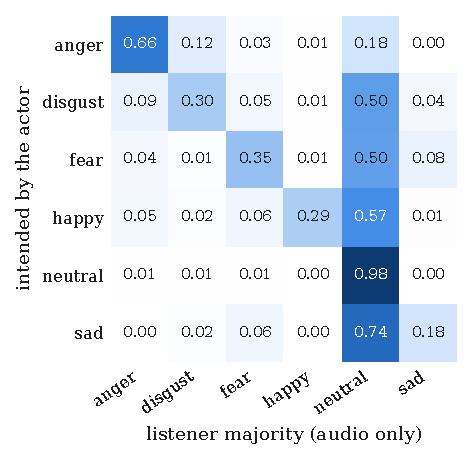
\includegraphics[width=\linewidth]{figures/listeners.pdf}
  \end{minipage}\hfill
  \begin{minipage}[c]{0.53\linewidth}
    \caption{Intended emotion (rows) vs.\ the audio-only listener majority (columns),
    row-normalised, clips without a tied vote. Listeners default to ``neutral'': 74\% of sad
    and 57\% of happy portrayals are heard as neutral. Anger is the most audible emotion.}
    \label{fig:listeners}
  \end{minipage}
\end{figure}

\paragraph{The main confound is the speaker.} A person's voice (pitch, timbre, habits) varies
more between people than between one person's emotions. Any split in which an actor appears on
both sides lets a model partly recognise \emph{who} instead of \emph{how}. All headline
numbers therefore use speaker-disjoint folds; a deliberately leaky random split is run only
to measure the leak.

\paragraph{Noise.} Additive noise comes from the \texttt{noise/} part of MUSAN~\citep{snyder2015musan}
(774 files), split deterministically by file name into a training pool (70\%) and a test
pool (30\%) so that augmentation and test conditions never share a recording.

% ================================================================ 3 method
\section{Method}\label{sec:method}

\begin{figure}[t]
\centering
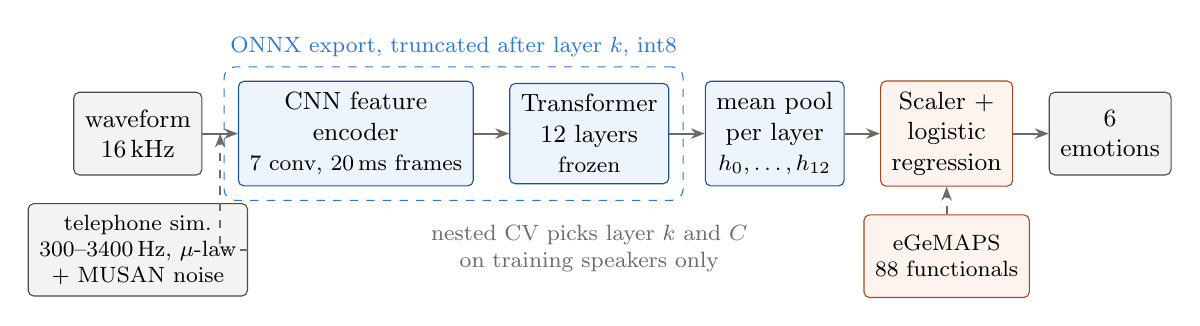
\begin{tikzpicture}[
  font=\small,
  box/.style={draw=#1!70!black, fill=#1!8, rounded corners=2pt, align=center,
              minimum height=1.05cm, inner sep=4pt},
  box/.default=seriesA,
  arr/.style={-{Stealth[length=5pt]}, thick, color=muted},
  node distance=0.45cm]
  \node[box=muted] (wav) {waveform\\16\,kHz};
  \node[box=muted, below=0.35cm of wav, font=\footnotesize] (tel) {telephone sim.\\300--3400\,Hz, $\mu$-law\\+ MUSAN noise};
  \node[box, right=of wav] (cnn) {CNN feature\\encoder\\{\footnotesize 7 conv, 20\,ms frames}};
  \node[box, right=of cnn] (tr) {Transformer\\12 layers\\{\footnotesize frozen}};
  \node[box, right=of tr] (pool) {mean pool\\per layer\\{\footnotesize $h_0,\dots,h_{12}$}};
  \node[box=seriesB, right=of pool] (probe) {Scaler +\\logistic\\regression};
  \node[box=muted, right=of probe] (out) {6\\emotions};
  \draw[arr] (wav) -- (cnn); \draw[arr] (cnn) -- (tr); \draw[arr] (tr) -- (pool);
  \draw[arr] (pool) -- (probe); \draw[arr] (probe) -- (out);
  \draw[arr, dashed] (tel.east) -| ($(wav.east)!0.5!(cnn.west)$);
  \node[box=seriesB, below=0.35cm of probe, font=\footnotesize] (ege) {eGeMAPS\\88 functionals};
  \draw[arr, dashed] (ege) -- (probe);
  \begin{scope}[on background layer]
    \node[draw=seriesA, dashed, rounded corners=4pt, fit=(cnn)(tr), inner sep=5pt,
          label={[font=\footnotesize,color=seriesA]above:{ONNX export, truncated after layer $k$, int8}}] {};
  \end{scope}
  \node[below=0.4cm of tr, font=\footnotesize, color=muted, align=center] {nested CV picks layer $k$ and $C$\\on training speakers only};
\end{tikzpicture}
\caption{Pipeline. The encoder is never fine-tuned; only a linear probe is trained. Dashed
branches are the experimental conditions: a simulated telephone channel before the encoder,
the eGeMAPS baseline replacing the encoder, and the CPU export of the truncated encoder.}
\label{fig:pipeline}
\end{figure}

\paragraph{Encoders and features.} We use the frozen \texttt{microsoft/wavlm-base-plus} and
\texttt{facebook/hubert-base-ls960} checkpoints (95M parameters each, pinned revisions). The
convolutional front-end turns the waveform into 50 frames per second; 12 transformer layers
follow. For each clip we average every hidden state over time, obtaining 13 vectors
$h_0,\dots,h_{12}\in\mathbb{R}^{768}$ ($h_0$ is the transformer input). Clips are processed one
by one: the front-end's group normalisation is sensitive to padding.

\paragraph{Probe and validation.} The classifier is \texttt{StandardScaler} + multinomial
logistic regression. The outer loop has five folds of \texttt{StratifiedGroupKFold} with
speakers as groups (stratified by sex). An inner loop of three speaker-grouped folds, run only
on the outer training speakers, selects the layer and the regularisation $C$; the reported
predictions never see the test speakers, neither in training nor in model selection. The
metric is UAR (balanced accuracy). Uncertainty is a 95\% percentile bootstrap over
\emph{speakers} (1{,}000 resamples), and models evaluated on the same clips are compared with a
paired bootstrap of the difference. The intervals cover test-speaker variability, not training
randomness (seed, fold assignment).

\paragraph{Telephone channel.} Band-pass 300--3400\,Hz, resampling to 8\,kHz, 8-bit $\mu$-law
companding and back to 16\,kHz; MUSAN noise is added before the channel at 20, 10 and 5\,dB
SNR. Probe A is trained on clean embeddings; probe B on embeddings of clips passed through a
randomly drawn channel condition with training-pool noise, deterministic per clip. The encoder
is identical in A and B.

\paragraph{CPU deployment.} The encoder, truncated after the layer chosen in Q1 and followed
by mean pooling, is exported with \texttt{torch.onnx} (dynamo) and quantised with ONNX
Runtime dynamic int8 quantisation (MatMul weights). Latency is measured for a 3\,s clip on a
laptop CPU (Intel i7-10850H, AVX2, no VNNI), 1 and 4 threads, 20 warm-up and 200 timed runs.

\paragraph{Comparing representations without coordinates.} The coordinates of an embedding are
arbitrary: replacing $X$ by $XQ$ for an orthogonal $Q\in O(d)$ and the next layer's weights by
$Q^\top W$ computes the same function. Two representations are therefore compared on the
\emph{orbits} of this group action, never element-wise. We use four tools, all on centred,
standardised embeddings $X,Y\in\mathbb{R}^{n\times d}$ of the same $n$ clips:
\begin{itemize}[leftmargin=1.4em]
\item \emph{Linear CKA}~\citep{kornblith2019cka}, the normalised Hilbert--Schmidt independence
      criterion~\citep{gretton2005hsic} with linear kernels,
      $\mathrm{CKA}(X,Y)=\|Y^\top X\|_F^2/(\|X^\top X\|_F\,\|Y^\top Y\|_F)$, invariant to
      rotations and isotropic scaling.
\item \emph{Orthogonal Procrustes}~\citep{schonemann1966procrustes},
      $\min_{Q\in O(d)}\|X-YQ\|_F^2 = 2-2\,\mathrm{tr}\,\Sigma$ for unit-norm $X,Y$ and
      $Y^\top X=U\Sigma V^\top$ (optimum $Q=UV^\top$): the distance between orbits.
\item \emph{Emotion subspaces on the Grassmann manifold.} The deviations of the six class means
      from the grand mean span a subspace $\mathcal{S}\subset\mathbb{R}^{768}$ of dimension 5,
      i.e.\ a point of $\mathrm{Gr}(5,768)=O(768)/\bigl(O(5)\times O(763)\bigr)$. Two subspaces
      are compared by the geodesic distance $d(\mathcal{S}_1,\mathcal{S}_2)=(\sum_i\theta_i^2)^{1/2}$,
      where $\theta_i$ are the principal angles~\citep{edelman1998geometry}; it is 0 for the same
      subspace and at most $\tfrac{\pi}{2}\sqrt5\approx3.51$. Across models, HuBERT is first rotated
      onto WavLM by Procrustes (no labels). To avoid fitting noise, the rotation is fitted on one
      random half of the actors and the subspaces are compared on the other half; the distance
      between the two halves of the \emph{same} model is the sampling noise floor.
\item \emph{Separability.} The Euclidean between/within ratio inside the class-mean subspace
      ignores the shape of the class clouds; the Fisher--LDA criterion
      $J=\mathrm{tr}(S_W^{-1}S_B)$, with the pooled within-class covariance $S_W$ estimated with
      Ledoit--Wolf shrinkage~\citep{ledoit2004shrinkage}, measures separation in the Mahalanobis
      geometry that a linear classifier actually exploits.
\end{itemize}

% ================================================================ 4 results
\section{Results}\label{sec:results}

\subsection{Q1--Q2: emotion in frozen layers, and the classical baseline}

\begin{table}[t]
\centering
\caption{Six-class emotion recognition on CREMA-D (chance 0.167). UAR with 95\% speaker-bootstrap
intervals; differences are paired, in percentage points. ``Leak'' = random split minus speaker
split. Layers are those chosen by the inner loop in the five outer folds.}
\label{tab:main}
\small
\begin{tabular}{@{}lcccc@{}}
\toprule
Features & UAR, speaker-indep. & UAR, random split & Leak, pp & Chosen layer \\
\midrule
eGeMAPS (88 functionals) & \ci{0.520}{0.501}{0.539} & -- & -- & -- \\
HuBERT Base, linear probe & \ci{0.714}{0.693}{0.736} & \ci{0.735}{0.717}{0.752} & \ci{+2.0}{+0.8}{+3.2} & 6, 7, 11, 11, 11 \\
WavLM Base+, linear probe & \ci{\textbf{0.751}}{0.733}{0.770} & \ci{0.768}{0.751}{0.784} & \ci{+1.6}{+0.7}{+2.5} & 6, 6, 7, 7, 7 \\
\midrule
WavLM $-$ HuBERT, pp & \ci{+3.7}{+2.5}{+4.9} & & & \\
WavLM $-$ eGeMAPS, pp & \ci{+23.2}{+21.8}{+24.6} & & & \\
\bottomrule
\end{tabular}
\end{table}

\begin{figure}[t]
  \centering
  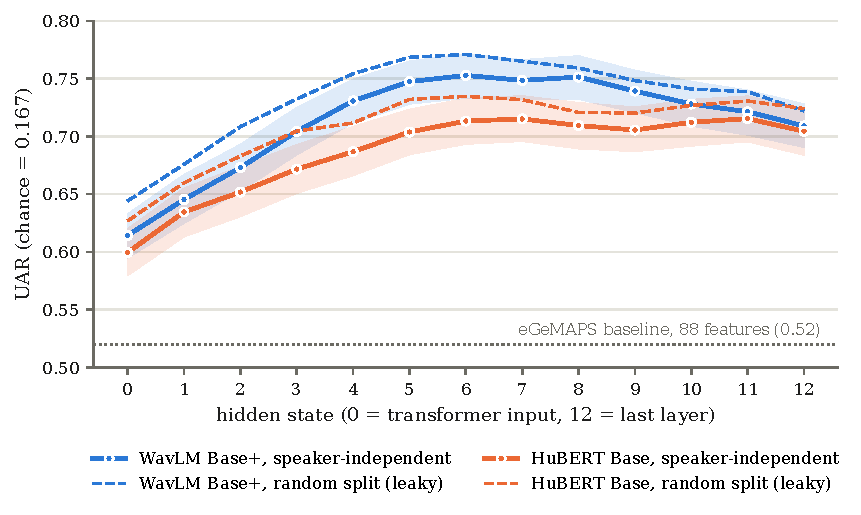
\includegraphics[width=0.86\linewidth]{figures/layers.pdf}
  \caption{UAR of the probe trained on each hidden state separately (speaker-independent folds,
  shaded 95\% intervals; dashed: the leaky random split). Emotion is most linearly accessible
  in the middle of the network; the last layer is worse. Even the transformer input $h_0$ beats
  the expert features.}
  \label{fig:layers}
\end{figure}

A frozen encoder with a linear probe reaches a UAR of 0.75 on unseen speakers
(\cref{tab:main}). The profile over layers (\cref{fig:layers}) rises to a plateau at layers 5--8
for WavLM and falls towards the output, consistent with layer-wise analyses showing that the
top layers of masked-prediction models specialise towards the pre-training targets
\citep{pasad2021layerwise}. The inner loop chose layer 6 or 7 in every WavLM fold, but HuBERT's
flatter profile makes its choice unstable (6--11). WavLM is better than HuBERT by
3.7\pp{} in a paired comparison.

\emph{Leakage} through the speaker is real but small for a linear probe (1.6--2.0\pp): the inner
loop always selected strong regularisation ($C=0.01$), which prevents memorising voices. A more
flexible head or fine-tuning would be expected to leak more, so speaker-disjoint splits remain
mandatory.

\emph{Is the large model needed?} Yes: under the identical protocol and folds, the 88 eGeMAPS
functionals reach 0.520, i.e.\ 23\pp{} less (\cref{fig:confusions,fig:rose}). The classical
features are closest on sadness, which is low-arousal and visible in pitch and loudness, and
furthest on disgust and neutral, which differ more in voice quality and articulation. This
matches the common observation that acoustics capture arousal well and valence poorly.
(Caveat: the inner loop mostly picked the largest $C$ of the grid for eGeMAPS; the grid was not
widened after the run.)

\begin{figure}[t]
  \centering
  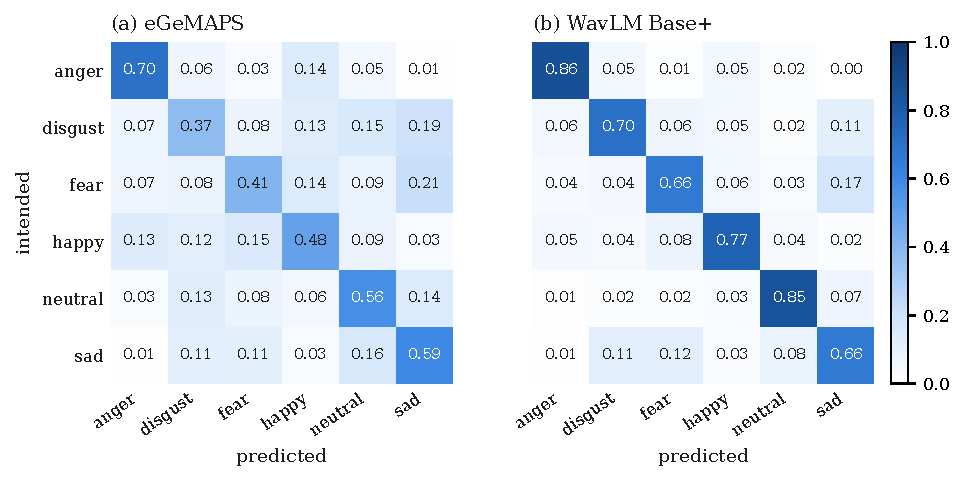
\includegraphics[width=0.92\linewidth]{figures/confusions.pdf}
  \caption{Row-normalised confusion matrices, speaker-independent out-of-fold predictions.
  The diagonal is the per-class recall.}
  \label{fig:confusions}
\end{figure}

% ---- the emotion rose: per-class recall drawn as Grandi's rose
\newcommand{\petal}[4]{%
  \fill[seriesA, fill opacity=0.28, draw=seriesA, draw opacity=0.9, line width=0.6pt]
    plot[domain=-30:30, samples=50, smooth] ({#1+\x}:{3.2*#3*cos(3*\x)}) -- cycle;
  \fill[seriesB, fill opacity=0.45, draw=seriesB!80!black, line width=0.6pt]
    plot[domain=-30:30, samples=50, smooth] ({#1+\x}:{3.2*#2*cos(3*\x)}) -- cycle;
  \node[font=\footnotesize, align=center] at (#1:3.75) {#4\\[-1pt]{\color{seriesB}#2}\,$\to$\,{\color{seriesA}#3}};
}
\begin{figure}[t]
\centering
\begin{minipage}[c]{0.46\linewidth}
\centering
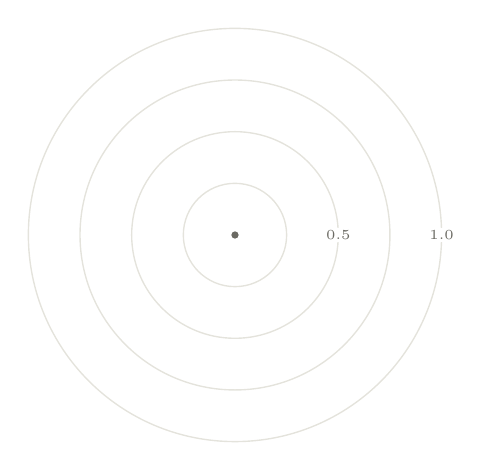
\begin{tikzpicture}[scale=0.82]
  \foreach \r in {0.25,0.5,0.75,1.0} \draw[gridc, line width=0.5pt] (0,0) circle (3.2*\r);
  \foreach \r in {0.5,1.0} \node[font=\tiny, color=muted, fill=white, inner sep=1pt] at (0:3.2*\r) {\r};
  % Generated by experiments/make_figures.py from the exp04 summary.json -- do not edit.
% \petal{angle}{eGeMAPS recall}{WavLM recall}{label}
\newcommand{\recallpetals}{%
\petal{90}{0.70}{0.86}{anger}%
\petal{30}{0.37}{0.70}{disgust}%
\petal{-30}{0.41}{0.66}{fear}%
\petal{-90}{0.48}{0.77}{happy}%
\petal{-150}{0.56}{0.85}{neutral}%
\petal{150}{0.59}{0.66}{sad}%
}

  \recallpetals
  \fill[muted] (0,0) circle (1.6pt);
\end{tikzpicture}
\end{minipage}\hfill
\begin{minipage}[c]{0.5\linewidth}
\caption{The emotion rose. Each petal is one lobe of Grandi's rose
$r(\theta)=\ell_k\cos\bigl(3(\theta-\theta_k)\bigr)$, $|\theta-\theta_k|\le30^\circ$, whose
length $\ell_k$ is the recall of class $k$: eGeMAPS ({\color{seriesB}orange}) inside WavLM Base+
({\color{seriesA}blue}). Circles mark recall 0.25, 0.5, 0.75, 1. The gap is smallest for
\emph{sad} and largest for \emph{disgust}.}
\label{fig:rose}
\end{minipage}
\end{figure}

\paragraph{Model vs.\ listeners.} On clips with a unique listener majority, the model agrees
with the intended label (UAR \ci{0.754}{0.736}{0.774}) far more often than listeners do
(\ci{0.461}{0.438}{0.487}), and with the listeners less often (\ci{0.604}{0.585}{0.623}). This is
\emph{not} super-human perception: the probe is trained on the acting conventions of 70+ actors
of this corpus, while each listener hears every actor for the first time. Subgroups behave as
expected: UAR grows with portrayed intensity (0.67, 0.72, 0.75 for low, medium, high on
sentence IEO), and the female--male difference (+3.4\pp, interval $-0.5$ to $+7.1$) is not
resolved by this sample.

\subsection{Q3: telephone channel and noise}

\begin{figure}[t]
  \centering
  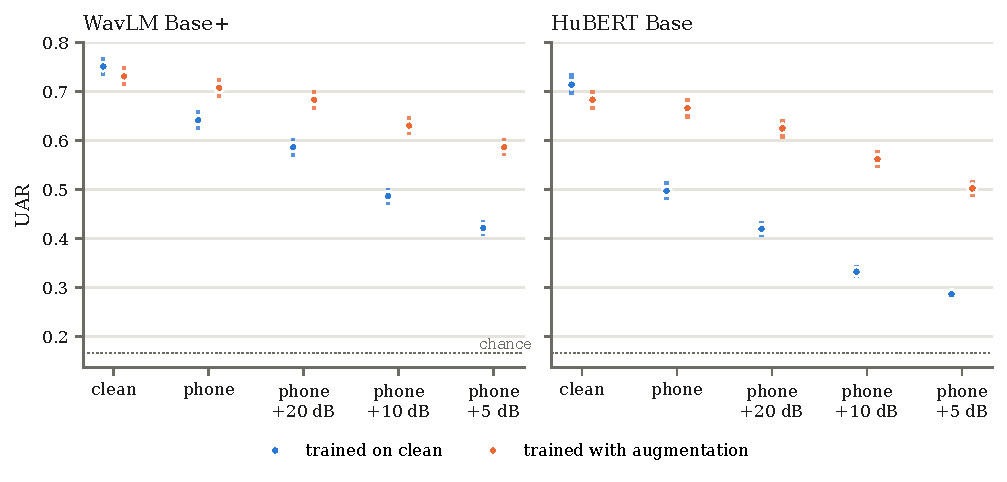
\includegraphics[width=0.95\linewidth]{figures/channel.pdf}
  \caption{UAR under simulated telephone conditions (95\% intervals). Blue: probe trained on
  clean audio (A); orange: probe trained with channel-and-noise augmentation (B). The encoder
  is the same frozen network in both.}
  \label{fig:channel}
\end{figure}

\begin{table}[t]
\centering
\caption{Cost of the telephone channel (drop of probe A relative to clean audio) and the gain
of augmentation (B $-$ A), in percentage points, paired 95\% intervals.}
\label{tab:channel}
\small
\begin{tabular}{@{}lcccc@{}}
\toprule
& \multicolumn{2}{c}{WavLM Base+} & \multicolumn{2}{c}{HuBERT Base} \\
\cmidrule(lr){2-3}\cmidrule(l){4-5}
Test condition & drop of A & gain B $-$ A & drop of A & gain B $-$ A \\
\midrule
clean & -- & \ci{$-$2.0}{$-$2.9}{$-$1.0} & -- & \ci{$-$3.1}{$-$4.2}{$-$2.1} \\
phone & \ci{10.9}{9.4}{12.4} & \ci{+6.6}{+5.3}{+8.0} & \ci{21.7}{19.8}{23.7} & \ci{+16.9}{+15.1}{+18.7} \\
phone + noise 20\,dB & \ci{16.4}{15.2}{17.7} & \ci{+9.7}{+8.5}{+10.9} & \ci{29.4}{27.5}{31.4} & \ci{+20.5}{+18.7}{+22.2} \\
phone + noise 10\,dB & \ci{26.4}{24.8}{28.1} & \ci{+14.4}{+12.9}{+15.8} & \ci{38.2}{36.2}{40.3} & \ci{+23.0}{+21.4}{+24.4} \\
phone + noise 5\,dB & \ci{32.9}{31.4}{34.5} & \ci{+16.5}{+15.1}{+17.9} & \ci{42.8}{40.8}{44.8} & \ci{+21.6}{+20.0}{+23.1} \\
\bottomrule
\end{tabular}
\end{table}

The channel alone, without any noise, removes 11\pp{} of WavLM's UAR and 22\pp{} of HuBERT's
(\cref{fig:channel}, \cref{tab:channel}). HuBERT was pre-trained on clean read audiobooks only,
WavLM on more diverse data with simulated noise and overlapping speech~\citep{chen2022wavlm};
the difference in robustness is consistent with that. Augmenting only the probe recovers
7--17\pp{} for WavLM at the price of 2\pp{} on clean audio---a trade worth making for calls.
The best layer moves slightly deeper under the channel (7 for every telephone condition).

\subsection{Q4: CPU deployment}

\begin{figure}[t]
  \centering
  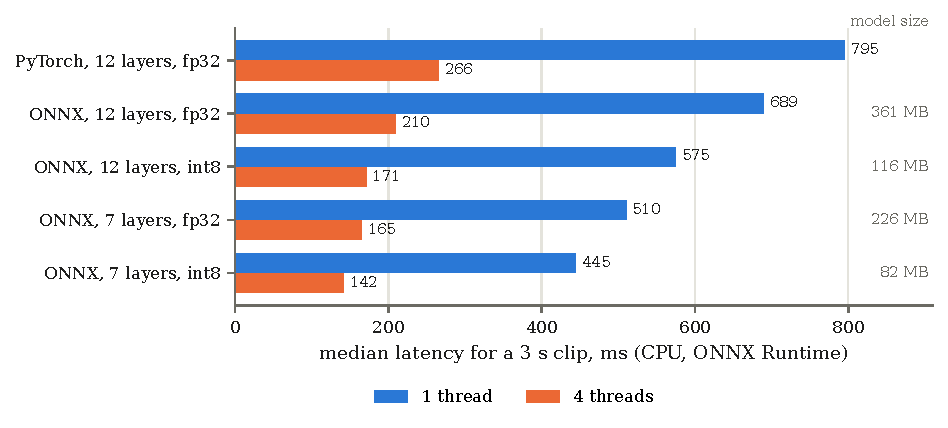
\includegraphics[width=0.86\linewidth]{figures/compression.pdf}
  \caption{Median latency of the WavLM encoder for a 3\,s clip on a laptop CPU, and ONNX model
  size. Truncation after layer 7 (chosen in Q1) does as much as int8 quantisation, without
  any loss of quality.}
  \label{fig:compression}
\end{figure}

ONNX export is exact (maximum absolute embedding difference $3.1\times10^{-6}$, threshold
$10^{-4}$) and by itself $1.15\times$ faster than PyTorch (\cref{fig:compression}). Truncating after
layer 7---a direct consequence of the layer analysis---gives $1.35\times$ and costs no
quality. Dynamic int8 quantisation shrinks the model $2.75\times$ but speeds it up only
$1.15\times$ (1 thread) and costs \ci{$-$0.7}{$-$1.3}{$-$0.1}\pp{} of UAR (93.1\% of predictions
unchanged, mean embedding cosine 0.992); \textbf{both pre-registered int8 criteria fail}.
The ONNX Runtime profiler explains why: in the truncated fp32 model, convolutions of the
front-end take 47\% of the time and remain in fp32 under dynamic quantisation (55\% of the int8
model's time), and a CPU without VNNI accelerates int8 matrix products only modestly.
Combined, PyTorch $\to$ ONNX + truncation + int8 yields $1.79\times$ (1 thread) and a model
4.4$\times$ smaller (82\,MB).

\subsection{Q5: the geometry of emotion representations}

\begin{figure}[t]
  \centering
  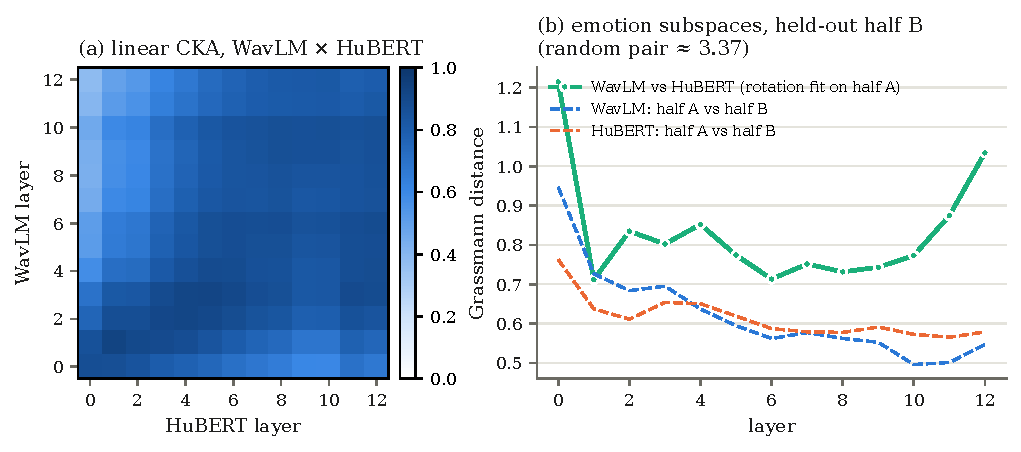
\includegraphics[width=0.95\linewidth]{figures/representations.pdf}
  \caption{(a) Linear CKA between all layers of WavLM and HuBERT. (b) Grassmann distance between
  the 5-dimensional emotion subspaces on the held-out half of the actors: across models after
  a Procrustes rotation fitted on the other half (green), and the sampling noise floor of each
  model (dashed). Two random 5-dimensional subspaces of $\mathbb{R}^{768}$ are 3.37 apart.}
  \label{fig:representations}
\end{figure}

\paragraph{The two encoders are similar up to rotation.} Corresponding layers have linear CKA of
0.80--0.92 (\cref{fig:representations}a); similarity is highest near the input and decreases
only mildly with depth.

\paragraph{Emotion lives in nearly the same subspace.} After rotating HuBERT onto WavLM on half of
the actors, the emotion subspaces on the other half are 0.71--0.85 apart in layers 4--9,
compared to a noise floor of 0.55--0.64 between two halves of the same model and 3.37 for random
subspaces (\cref{fig:representations}b). Up to sampling noise and a rotation, both models put the
six emotion means in almost the same five directions.

\paragraph{So why is WavLM better?} The obvious hypothesis---WavLM separates the class means more
cleanly---is refuted: the Euclidean between/within ratio is even \emph{higher} for HuBERT in the
middle layers, and decreases with depth in WavLM while UAR increases (\cref{fig:fisher}a). The
Fisher--LDA criterion, which accounts for the shape of the within-class scatter, tracks the
layer-wise UAR closely: $r=0.92$ for WavLM and $0.97$ for HuBERT (\cref{fig:fisher}b), and is
higher for WavLM in every layer from 1 to 10. The variance decomposition (\cref{fig:variance})
completes the picture: going deeper, the share of variance explained by the speaker falls
(0.25 $\to$ 0.10 in WavLM) and the share explained by the sentence rises (0.08 $\to$ 0.39 at layer
9), while the share explained by emotion shrinks. Emotion does not become ``louder'' in the middle
layers; it becomes better separated \emph{relative to} the within-class variation left by speaker
and sentence, which is exactly what $J$ measures. These analyses are descriptive and were not validated on held-out data beyond the
split-half control.

\begin{figure}[t]
  \centering
  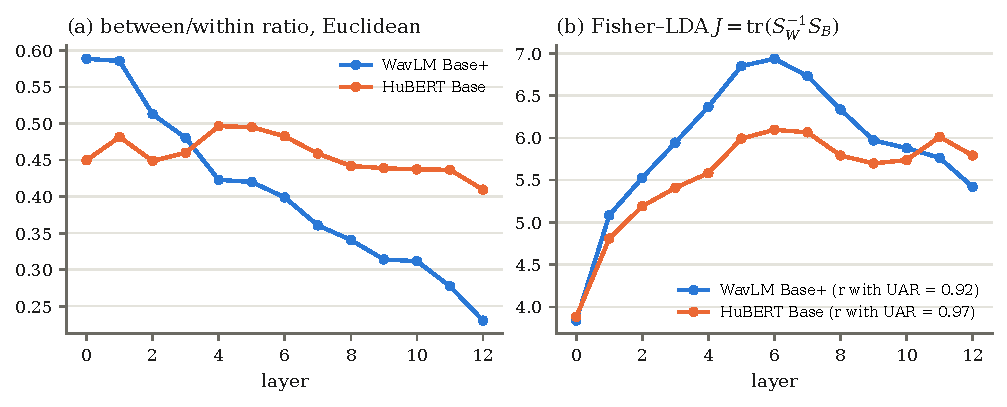
\includegraphics[width=0.92\linewidth]{figures/fisher.pdf}
  \caption{Class separability by layer. (a) Euclidean between/within ratio in the class-mean
  subspace. (b) Fisher--LDA criterion with Ledoit--Wolf shrinkage; $r$ is the Pearson correlation
  of the curve with the layer-wise UAR of \cref{fig:layers}.}
  \label{fig:fisher}
\end{figure}

\begin{figure}[t]
  \centering
  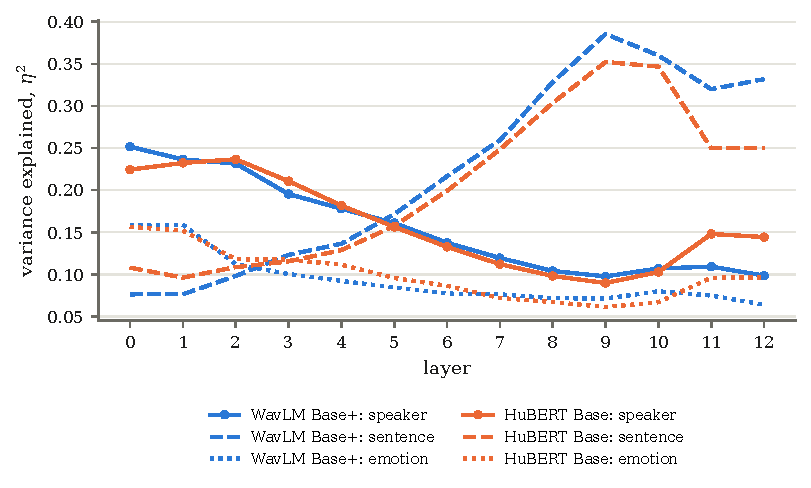
\includegraphics[width=0.78\linewidth]{figures/variance.pdf}
  \caption{Share of embedding variance explained by speaker, sentence and emotion ($\eta^2$ of
  standardised dimensions, averaged), by layer.}
  \label{fig:variance}
\end{figure}

% ================================================================ 5 criteria & discussion
\section{Pre-registered criteria}

\begin{table}[!htb]
\centering
\caption{Success criteria fixed before the runs (\texttt{docs/PREREGISTRATION.md}) and their
verdicts, computed by \texttt{experiments/make\_report.py} from the run logs.}
\label{tab:criteria}
\small
\begin{tabularx}{\linewidth}{@{}lXlc@{}}
\toprule
Stage & Criterion & Value & Verdict \\
\midrule
1 & Speaker-independent UAR: lower 95\% bound $>1/6$ & $0.733>0.167$ & met \\
1 & Leakage: lower bound of paired (random $-$ speaker) $>0$ & $+0.7$\pp & met \\
2 & Drop on telephone conditions reported with paired intervals & \cref{tab:channel} & met \\
2 & Augmentation: lower bound of B $-$ A $>0$ on all telephone conditions & min.\ $+5.3$\pp & met \\
3 & ONNX $\equiv$ PyTorch: max.\ abs.\ difference $\le10^{-4}$ & $3.1\times10^{-6}$ & met \\
3 & int8: lower bound of UAR(int8) $-$ UAR(fp32) $\ge-1$\pp & $-1.26$\pp & \textbf{not met} \\
3 & int8: p50 latency reduced at least $1.5\times$ & $1.15\times$ & \textbf{not met} \\
add. & WavLM beats eGeMAPS: lower bound of paired difference $>0$ & $+21.8$\pp & met \\
\bottomrule
\end{tabularx}
\end{table}

\section{Discussion and limitations}

\paragraph{What transfers to telephone triage.} (1) Speaker-disjoint validation is
non-negotiable, and the leak grows with the capacity of the head. (2) The telephone channel, not
the classifier, is the main threat; encoder choice (WavLM) and channel augmentation address it
cheaply. (3) Layer analysis is not only diagnostic: it directly yields a 1.35$\times$ faster and
smaller deployable model. (4) Quantisation must be profiled on the target hardware before it is
promised: here the front-end convolutions, not the transformer, are the bottleneck.

\paragraph{Limitations.} Acted emotions are not real calls: actors read 12 fixed sentences with
often exaggerated portrayals in studio conditions, and the labels are what the actor intended.
The numbers compare methods; they are not clinical accuracy. The channel simulation is simplified
(continuous $\mu$-law instead of table-based G.711, no mobile codecs such as AMR or Opus, no packet
loss or echo). Latency was measured on a single laptop CPU; server CPUs with VNNI usually gain
more from int8. Intervals do not include training randomness. All analyses use English speech
from one corpus.

\paragraph{Next steps.} Static (calibrated) quantisation of the convolutional front-end or a
distilled front-end~\citep{chang2022distilhubert}; measurement on a VNNI server CPU; streaming
inference with sliding windows; validation on a second acted corpus and on naturalistic,
non-English telephone speech.

\section{Conclusion}

A frozen WavLM Base+ with a linear probe recognises six acted emotions on unseen speakers with a
UAR of 0.75, far above expert acoustic features, with emotion concentrated in the middle layers.
A telephone channel is the dominant degradation and is largely recoverable by augmenting the probe.
For CPU inference, truncation guided by the layer analysis beats int8 quantisation on this
hardware. Two differently trained encoders encode emotion in nearly the same subspace; what makes
one better is the geometry of the scatter around the class means.

\paragraph{Reproducibility.} Code, configuration and tests are at the repository above. Each run
writes its configuration and git commit next to its results; the README tables, the verdicts
in \cref{tab:criteria} and all figures in this report are regenerated from those run logs by
\texttt{experiments/make\_report.py} and \texttt{experiments/make\_figures.py}. No audio is
redistributed. The title page margin is drawn procedurally by the \texttt{florilegium}
package~\citep{florilegium}.

{\small
\bibliographystyle{abbrvnat}
\bibliography{refs}
}

\vspace{1em}
\begin{center}\florilegiumornament[size=2.2em]{flower}\end{center}

\end{document}
